%\documentclass[oribibl,runningheads,a4paper]{llncs}
\documentclass[a4paper]{llncs}
\usepackage{url}
\usepackage{times}
\usepackage{listings}
\usepackage{graphicx,marvosym}

\newcommand{\comment}[1]{}
\newcommand{\citenot}[1]{}
\newcommand{\blurb}[1]{{\texttt{[.. #1..]}}}


\begin{document}

\lstdefinestyle{nonumbers}
{numbers=none}
\lstset{language=C,basicstyle=\small}
\lstset{numbers=left, numberstyle=\tiny, stepnumber=1, numbersep=5pt}
\lstset{tabsize=2}
\lstset{firstnumber=1}
\lstset{frame=single}
\lstset{
  language={C},
  morekeywords={assert,uchar,class}
}

%\mainmatter  % start of an individual contribution

\title{SMT-Based Bounded Model Checking of C++ Programs}
%\subtitle{(Competition Contribution)}
%\titlerunning{}
\author{Mikhail Ramalho$^1$ 	\and
	Felipe Rodrigues$^1$   	\and
	Hendrio Marques$^1$   	\and
	Mauro Freitas$^1$   	\and
	Lucas Cordeiro$^1$   	\and
	Bernd Fischer$^2$}
\authorrunning{Mikhail Ramalho, Felipe Rodrigues, Hendrio Marques, Mauro Freitas, Lucas Cordeiro, Bernd Fischer}
\institute{
  $^1$ Electronic and Information Research Center, %\\
  Federal University of Amazonas, Brazil\\
  %\url{lucascordeiro@ufam.edu.br}
  %\\\smallskip
  $^2$ Electronics and Computer Science, %\\
  University of Southampton, UK\\
  %\url{{jcmm106,dan,bf}@ecs.soton.ac.uk}
  %\url{http://www.ecs.soton.ac.uk}
  \url{esbmc@ecs.soton.ac.uk}
}

\maketitle

\begin{abstract}
Bounded Model Checking (BMC) of C++ programs presents greater
complexity than that of C programs due to the features that the language offers, such as
templates, containers, and exception handling.\ We present ESBMC++, a bounded
model checker for C++ programs, which encodes the verification conditions
using different background theories supported
by an SMT Solver.\ ESBMC++ uses an operational model,
an abstract representation of
the standard C++ libraries, which conservatively approximates their semantics.\ Our
experimental results show that our approach can handle a wider range of the C++
constructs than existing approaches and substantially reduce the verification time.
\end{abstract}
%
%------------------------------
\section{Introduction}
%------------------------------
%
Bounded Model Checking (BMC) based on Boolean Satisfiability (SAT) solvers
has already been successfully applied to verify software and to discover
subtle errors in real systems~\cite{handbook09}.\ In an attempt to cope
with growing system complexity, SAT solvers are increasingly
replaced by Satisfiability Modulo Theories (SMT) solvers to prove the generated
verification conditions (VCs)~\cite{Armando09,Ganai06,Cordeiro12}.\
There have also been attempts to apply BMC to the verification of C++
programs~\cite{Florian12,Yang12} but with limited success. The main challenge here is to handle large
programs and to support the features that the languages offers, such as templates,
containers and exception handling.

C++ is widely used, but systems that use C++
tend to require a high verification effort. C++
verification involves many more challenges than that of plain ANSI-C since the language provides
a wider set of features (e.g., object-oriented programming), libraries (e.g., specialized
input-output), and functionalities (e.g., templates). In order to be attractive for mainstream software development,
C++ model checkers have to support these and at the same time maintain
high speed, accuracy, efficiency, and user-friendliness.


We propose to apply
BMC to C++ programs using an operational model,  which
is an abstract representation of the standard C++ libraries that
conservatively approximates their semantics. To support this operational model, we extended
our ESBMC tool~\cite{Cordeiro12} that in turn builds on
the front-end of CBMC \cite{Clarke04} to support C++ features such
as inheritance, polymorphism, templates, and exception handling.

We present a novel implementation of an operational model of the sequential STL
containers, its preconditions and simulation features (e.g., how we store the
elements values of the containers), and how these are used in order to verify
real-world C++ programs.  Additionally, we develop novel approaches to handle
exceptions in C++ programs (in particular, exception specification for
functions and methods) that previous approaches are not able to deal
with~\cite{PrabhuMBIG11,Blanc07,Florian12}.
%
%------------------------------
\section{Background and System Architecture}
%------------------------------

ESBMC++ builds on the front-end of CBMC to generate the VCs for a given C++ program,
and on the back-end of ESBMC to encode the VCs using different background theories
and SMT solvers.
%%% In this section, we describe the main features of CBMC that we use,
%%% and present the background theories used in the back-end of ESBMC.

%------------------------------------------------------ \subsection{C
%Bounded Model Checker} \label{02-CBoundedModelChecker}
\smallskip\noindent{\bf C Bounded Model Checker.}
%------------------------------------------------------
%
CBMC implements BMC for ANSI-C/C++ programs using SAT/SMT
solvers~\cite{Clarke04}.  It can process C/C++ code using the goto-cc
tool~\cite{Wintersteiger09}, which compiles the C/C++ code into
equivalent GOTO-programs (i.e., control-flow graphs) using a
gcc-compliant style. The GOTO-programs can then be processed by the
symbolic execution engine. Alternatively, CBMC uses its own, internal
parser based on Flex/Bison, to process the C/C++ files and to build an
abstract syntax tree (AST). The typechecker of CBMC's front-end
annotates this AST with types and generates a symbol table. CBMC's IRep
class then converts the annotated AST into an internal,
language-independent format used by the remaining phase of the
front-end.  ESBMC++ modifies this front-end to handle the definitions of
the standard C++ libraries and other the features (e.g., inheritance,
template, and exception handling) are treated internally.

CBMC (and ESBMC) use two recursive functions that compute the
\emph{constraints} $C$ (i.e., assumptions and variable assignments) and
\emph{properties} $P$ (i.e., safety conditions and user-defined
assertions). In addition, both tools automatically generate safety conditions
that check for example for arithmetic overflow and underflow, array bounds
violations, and NULL-pointer dereferences, in the spirit of Site's clean
termination~\cite{Sites74}. Both functions accumulate the control flow
predicates to each program point and use these predicates to guard both
the constraints and the properties, so that they properly reflect the
program's semantics. A VC generator (VCG) then derives the VCs from
these.

%------------------------------------------------------
%\subsection{Satisfiability Modulo Theories}
%\label{02-SatisfiabilityModuloTheories}
\smallskip\noindent{\bf Satisfiability Modulo Theories.}
%------------------------------------------------------
%
SMT decides the satisfiability of first-order formulae using a
combination of different background theories and thus generalizes
propositional satisfiability by supporting uninterpreted functions,
linear and non-linear arithmetic, bit-vectors, tuples, arrays, and other
decidable first-order theories. Given a theory ${\cal T}$ and a
quantifier-free formula $\psi$, we say that $\psi$ is $\cal
T$-satisfiable if and only if there exists a structure that satisfies
both the formula and the sentences of ${\cal T}$, or equivalently, if
${\cal T}\cup \{\psi\}$ is satisfiable~\cite{Bradley07}. Given a set
$\Gamma\cup \{\psi\}$ of formulae over $\cal T$, we say that $\psi$ is a
$\cal T$-consequence of $\Gamma$, and write $\Gamma\models_{\cal
T}\psi$, if and only if every model of ${\cal T}\cup\Gamma$ is also a
model of $\psi$.  Checking $\Gamma\models_{\cal T}\psi$ can be reduced
in the usual way to checking the $\cal T$-satisfiability of
$\Gamma\cup\{\neg\psi\}$.

%%% The SMT-LIB initiative~\cite{smtlib09} aims at establishing a common standard
%%% for the specification of background theories, but most SMT solvers provide functions
%%% in addition to those specified in the SMT-LIB. Therefore, we describe here the fragments
%%% that we found in the SMT solvers Boolector, CVC3, and Z3 for the theory of linear, non-linear,
%%% and bit-vector arithmetic. We summarize the syntax of these background theories as follows,
%%% using standard notations where appropriate:
%%%
%%% \[\begin{array}{r@{\:\:}c@{\:\:}l}
%%% \\[-5ex]
%%% \mathit{F}  & ::= & \mathit{F} \: \mathit{con} \: \mathit{F} \:
                    %%% | \: \neg\mathit{F} \:
                    %%% | \: A \\
%%% \mathit{con}  & ::= & \: \wedge \:
                    %%% | \: \vee \:
                    %%% | \: \oplus \:
                    %%% | \: \Rightarrow \:
                    %%% | \: \Leftrightarrow \: \\
%%% \mathit{A} & ::= &  \mathit{T} \: \mathit{rel} \: \mathit{T} \:
                    %%% | \: \mathit{Id} \: | \: true \: | \: false \\
%%% \mathit{rel}  & ::= & \: < \:
                    %%% | \: \leq \:
                    %%% | \: > \:
                    %%% | \: \geq
                    %%% | \: = \:
                    %%% | \: \neq \: \\
%%% \mathit{T}  & ::= &  \mathit{T} \: op \: \mathit{T} \:
                    %%% | \: \sim T \:
                    %%% | \: \mathit{ite}(\mathit{F}, \: \mathit{T}, \mathit{T}) \:
                    %%% | \: \mathit{Const} \:
                    %%% | \: \mathit{Id} \: | \\
              %%% &   & \mathit{Extract}(T, i, j)
                    %%% | \: \mathit{SignExt}(T, k)
                    %%% | \: \mathit{ZeroExt}(T, k) \\
%%% \mathit{op}   & ::= & + \:
                    %%% | \: - \:
                    %%% | \: * \:
                    %%% | \: / \:
                    %%%%%%  | \: rem \:
                    %%% | \: \texttt{<<} \:
                    %%% | \: \texttt{>>} \:
                    %%% | \: \texttt{\&} \:
                    %%% | \: \texttt{|} \:
                    %%% | \: \oplus \:
                    %%% | \: @ \:
%%% \end{array}
%%% \]
%%%
%%% \noindent
%%% Here, $F$ denotes Boolean-valued expressions with atoms $A$, and $T$ denotes terms
%%% built over integers, reals, and bit-vectors.
%%% %%% using the binary operators \emph{op}.
%%% The logical connectives $\mathit{con}$ consist of conjunction
%%% ($\wedge$), disjunction ($\vee$), exclusive-or ($\oplus$), implication
%%% ($\Rightarrow$), and equivalence ($\Leftrightarrow$).
%%% The bit-level operators are and
%%% (\texttt{\&}), or (\texttt{|}), exclusive-or ($\oplus$), complement ($\sim$),
%%% right-shift (\texttt{>>}), and left-shift (\texttt{<<}).
%%% $\mathit{Extract}\left(T, i,j\right)$ denotes bit-vector extraction from bits
%%% \textit{i} down to \textit{j} to yield a new bit-vector of size  $i-j+1$ while
%%% $@$ denotes the concatenation of the given bit-vectors.
%%% $\mathit{SignExt}\left(T, k\right)$ extends a bit-vector of size $w$
%%% to the signed
%%% equivalent bit-vector of size $w+k$,
%%% while $\mathit{ZeroExt}\left(T, k\right)$ extends the bit-vector
%%% with zeros to the unsigned equivalent bit-vector of size $w+k$. The conditional
%%% expression $\mathit{ite}(f, t_1, t_2)$ takes a Boolean formula $f$ and
%%% depending on its value selects either the second or the third argument.
%%% The interpretation of the
%%% relational operators (i.e., $<$, $\leq$, $>$, $\geq$), the non-linear
%%% arithmetic operators $*$, $/$, remainder (\emph{rem}) and the right-shift
%%% operator (\texttt{>>}) depends on whether their arguments are unsigned or
%%% signed bit-vectors, integers or real numbers.  The arithmetic operators
%%% induce checks to ensure that the arithmetic operations do not overflow
%%% and/or underflow.
%%%

%------------------------------------------------------
\smallskip\noindent{\bf Arrays and Tuples.}
%------------------------------------------------------
%
The most important theories for ESBMC are the array and tuple theories,
which are used to model container data structures and objects,
respectively.
The array theories of SMT solvers are typically based on the
McCarthy axioms~\cite{McCarthy62}. The function \emph{select(a, i)}
denotes the value of $a$ at index position $i$ and \emph{store(a, i, v)}
denotes an array that is exactly the same as array $a$ except that the
value at index position $i$ is $v$. %%% (if $i$ is within the array bounds).
Formally, the functions \emph{select} and \emph{store} can then be characterized
by the following two axioms~\cite{CVC07,Boolector09,Z08}:
%
\[
\begin{array}{l}
  i=j      \Rightarrow select\left(store\left(a,i,v\right),j\right)=v \\
  i \neq j \Rightarrow select\left(store\left(a,i,v\right),j\right)=select\left(a,j\right)
\end{array}
\]

\noindent
Array bounds checks need to be encoded separately, as the array theories
employ the notion of unbounded arrays size, but arrays in software are
typically of bounded size.

%%% \noindent Equality on array elements is defined by the theory of equality with uninterpreted
%%% functions (i.e., $a = b \wedge i = j \Rightarrow select\left(a,i\right) = select\left(b,j\right)$)
%%% and the extensional theory of arrays then allows reasoning about array equality as follows~\cite{CVC07,Boolector09,Z08}:
%%% \[
%%% \begin{array}{l}
  %%% a = b    \Leftarrow  \forall i \cdot select\left(a,i\right) = select\left(b,i\right)  \\
  %%% a \neq b \Rightarrow \exists i \cdot select\left(a,i\right) \neq select\left(b,i\right)
%%% \end{array}
%%% \]

Tuples %%% are used to model the ANSI-C union and struct datatypes. They
provide
\mbox{store} and \mbox{select} operations similar to those in arrays, but work
on the tuple \mbox{elements}. Each field of the tuple is represented by an
integer constant. Hence, the expression $\mathit{select}(t, f)$ denotes the field $f$
of tuple $t$ while the expression $\mathit{store}(t, f, v)$ denotes a tuple $t$
that at field $f$ has the value $v$ and all other fields remain the
same.

%------------------------------
\section{C++ Operational Model}
%------------------------------

%%% During the verification process, ESBMC++ has to identify all the
%%% specifications and features of the C++ program to generate the AST.
%%% The specifications are related to the definitions of the standard C++
%%% libraries such as classes, methods, and types while the features
%%% (e.g., inheritance, template, and exception handling) are treated internally
%%% in ESBMC++ in different levels (i.e., scan, parser, and type-check).
%%% In this sense, we developed a simplified representation of the C++ libraries
%%% called C++ Operational Model (COM) to represent the classes, methods,
%%% and other features. The development process of the COM can be split into
%%% two phases: \textit{structural} and \textit{modeling}. In the structural phase,
%%% we built a set of classes with a specific hierarchical relationship, the signature
%%% of their methods, and specific data. In the modeling phase, we focus on the pre-
%%% and post-conditions and how these are used to verify real-world programs that
%%% depend on the C++ libraries.

%------------------------------
%%% \subsection{Structure and Model}
%------------------------------

ESBMC++ relies on an operational model of the standard C++ libraries to
verify properties related to the definitions in the supported data
types.  We thus developed a simplified representation of the C++
libraries called the C++ Operational Model (COM), which represents the
classes, methods, and other features similar to the actual
structure~\cite{CppReference12}.  This operational model is inserted
into the verification process at the level of the source code (i.e.,
both model and program are passed as parameters at the beginning of the
verification process). The COM consists of four groups of libraries, as
shown in Figure~\ref{figure:cpp-diagram}: \emph{C libraries},
\emph{input/output stream}, \emph{standard template libraries}, and
\emph{general libraries}.

\begin{figure*}[ht] \centering
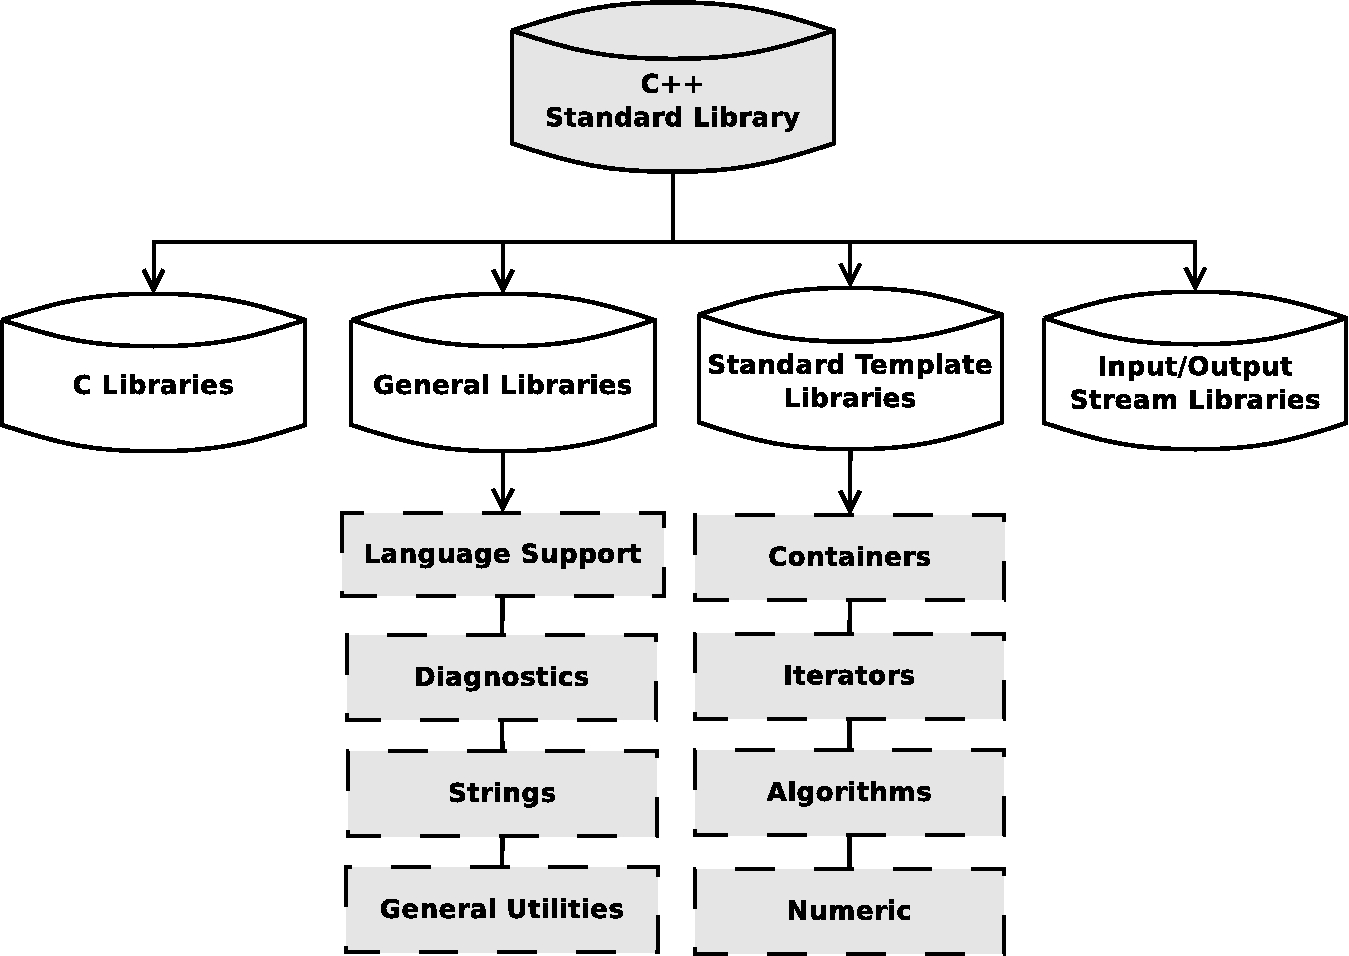
\includegraphics[scale=0.25]{figures/diagramascpp}
\caption{Configuration and functional classification of the operational model.}
\label{figure:cpp-diagram}
\end{figure*}

%------------------------------
\subsection{C Libraries}
%------------------------------

The standard C++ libraries also include all the ANSI-C libraries, which
are already supported by ESBMC.  However, for the verification of C++
programs, ESBMC++ follows a different path to parse the C++ programs.
For this reason, we also have to build a representation of the ANSI-C
libraries into the operational model; otherwise, ESBMC++ does not recognize
the methods of the library and fails.

\comment{
We can thus
define this libraries' set in a simplified structure, which consists
essentially of macro definitions and functions. From this ANSI-C libraries' set,
there are libraries that contains only macro definitions (e.g., the \textit{ciso646} library
defines a spelling set to the logic operators). To build the structure of this
library, we distingue between two kinds of spelling: macros and operators.
For convention, we assume the macros set $M$ as follows:
%
\begin{eqnarray}
\label{ciso646-macro-set}
\left\{and, and\_eq, bitand, bitor, compl, not, not\_eq, or, or\_eq, xor, xor\_eq\right\} \subset M
\end{eqnarray}

The operator set $O$ is defined as follows:
%
\begin{eqnarray}
\label{ciso646-operator-set}
\left\{
\: \&\&,
\: \&= \:,
\: \& \:,
\: | \:,
\: \widetilde{} \:,
\: ! \:,
\: || \:,
\: |= \:,
\:\: \widehat{} \:\:,
\: \widehat{}= \:
\right\} \subset O
\end{eqnarray}

Therefore, we define the syntax for these definitions sets as:
%
\begin{equation}
\left( \alpha \in M \wedge \beta \in O \right) \Rightarrow \left(\forall\alpha\right)\left(\exists\beta\right)\left(\alpha\equiv\beta\right)
\label{eq:csi646-definitions}
\end{equation}
}

Within the ANSI-C libraries set, we can also represent the structure
of others libraries with functions only. This is case of the \textit{csignal}
library, which deals with signals that are emitted to a given code.
We thus define that the operational model of this library can been represented
by signals that raise functions. For an array $a$ of size $N$ and
for a finite signals set $S$ where $\left\{s_{1},\ldots, s_{n}\right\}\:\subset\:S$
and $n < N$, the function signal records a certain function in one specific signal
such that when the raising function is called with the respective signal,
the registered function is called. Let $f$ be a function, $\sigma$ be a signal,
and $\eta$ be a NULL element. We can thus model $C$ and $P$
of the function $signal\left(\sigma, f\right)$ as:
%
\begin{equation}
\label{quantifier-free-formulae-sginal}
C := \left [ \begin{array}{ll}
                a' = store\left(a,\sigma,f\right) \\
              \end{array} \right ],  \\
P := \left [ \begin{array}{ll}
                \left(\sigma = s_{1}\right) \vee \ldots \vee \left(\sigma = s_{n}\right) \\
              \end{array} \right ]  \\
\end{equation}

%%\blurb{Shouldn't this call the function set by signal?}
The function $raise\left(\sigma\right)$ can be modeled in our operational model as:
%
\begin{equation}
\label{quantifier-free-formulae-raise}
C := \left [ \begin{array}{ll}
                f = select\left(a',\varphi\right) \\
              \end{array} \right ],  \\
P := \left [ \begin{array}{ll}
                \left(\varphi = s_{1}\right) \vee \ldots \vee \left(\varphi = s_{n}\right) \wedge \left(select\left(a',\varphi\right) \neq \eta\right) \\
              \end{array} \right ]  \\
\end{equation}
\vspace*{-4ex}
%---------------------------------------------
\subsection{Input/Output Stream Libraries}
%---------------------------------------------

To build the operational model, it is important
to define a class structure that is as close as to the
real implementation so that ESBMC++ can correctly identify
the relationships between classes in a given program and
then introduce such relationships to build the AST.
We have thus elaborated a hierarchical structure for the
input/output (I/O) stream library that is similar to the actual
one (as shown in Figure~\ref{figure:cpp-inputoutputdiagram}).
In our I/O stream operational model, the input operator $>>$
is simply modelled as a non-deterministic variable and we do not check
any safety property. Similarly, the output operator $<<$ does not
present any constraints or properties to be checked since
we do not check whether a given value has been printed on the screen
(ESBMC++ is interested in checking only the properties related to
software and not that of hardware).


\begin{figure*}[ht]
\centering
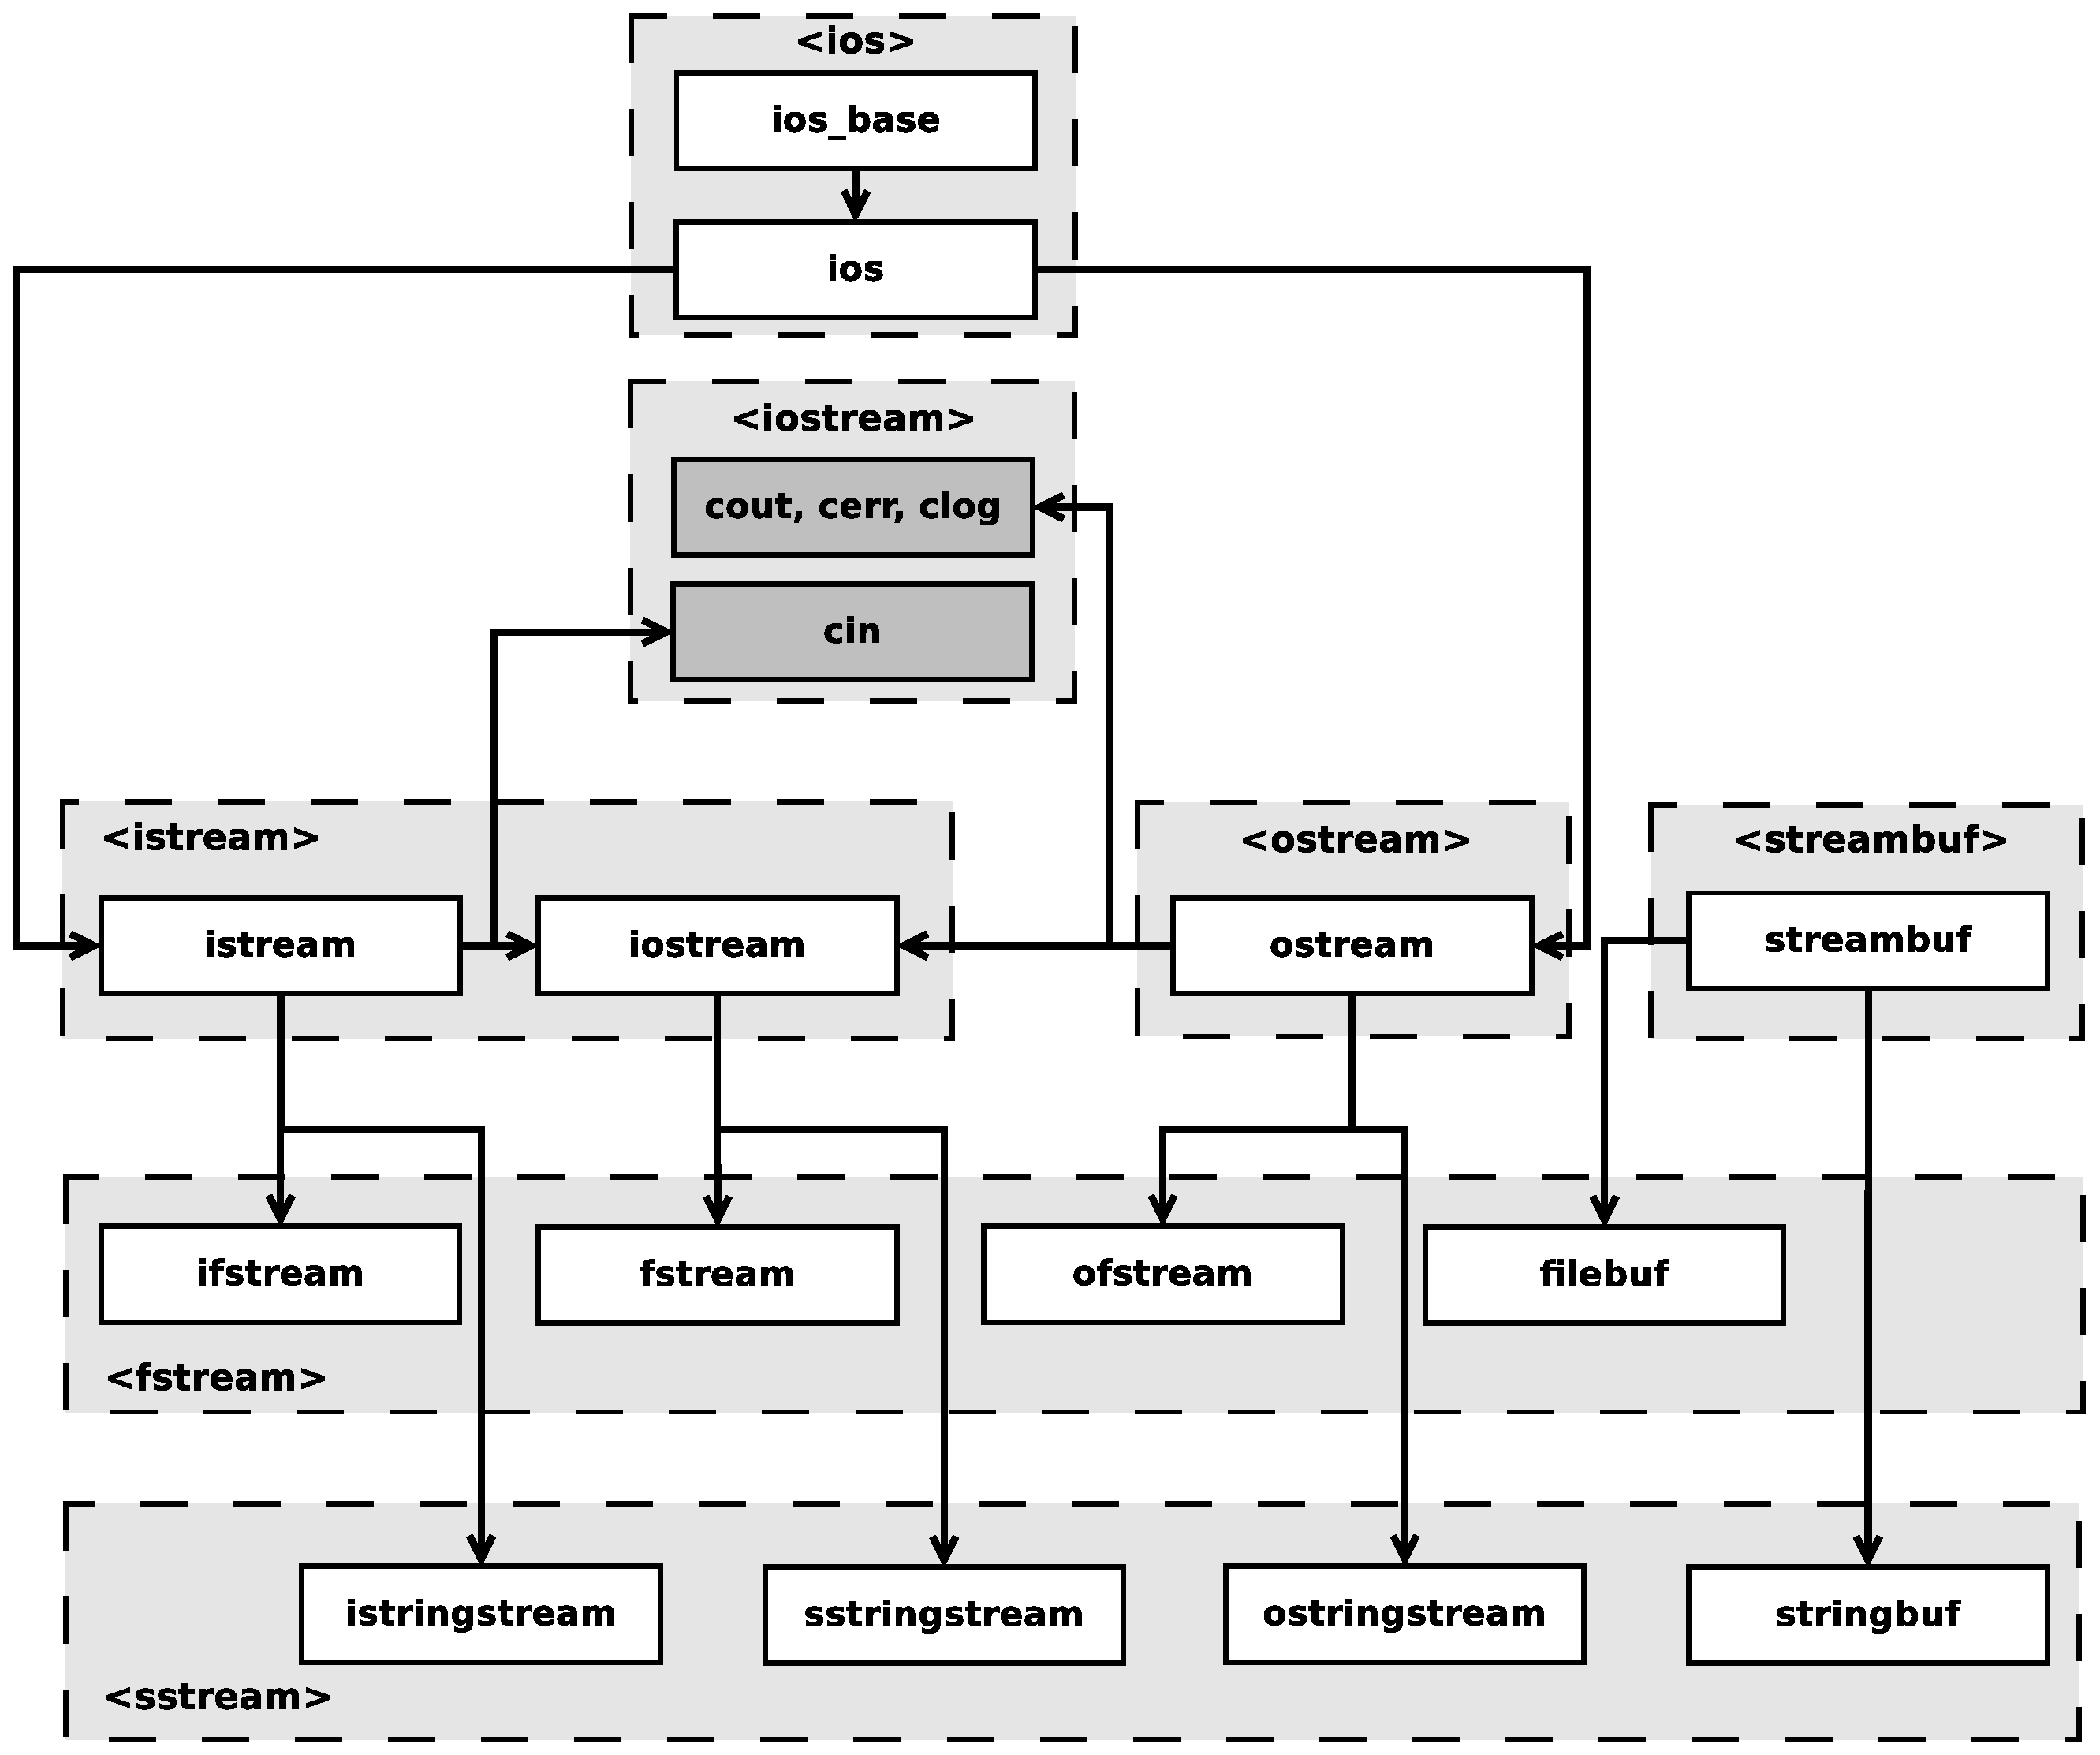
\includegraphics[scale=0.24]{figures/inputoutputdiagram}
\caption{Hierarchical structure of the Input / Output Stream Libraries.
Dotted gray square represents the library, white square represents the class and dark gray square represents the access objects.}
\label{figure:cpp-inputoutputdiagram}
\end{figure*}

%-------------------------------------------
\subsection{Standard Template Libraries}
%-------------------------------------------

\comment{The operational model
of the \textit{algorithms} library is composed by a set of algorithms
related to manipulation of STL containers, arrays, and string objects.
To given an idea of the basic operations of this library, we describe
the implemenation of the functions $find$ and $for\_each$ in our
operational model.

The function $find$ looks for a certain element within a range while the
function $for\_each$ applies a given function to a range. Let $\eta$ be
a $NULL$ element and $I$ be a range, such that $\left\{first, last, n, i\right\}\:\subset\:I$.
Here, $first$ represents the pointer to the beginning of the range, $last$ represents
the pointer to the ending of the range, $n$ represents the number of elements
contained between $first$ and $last$, $i$ represents a certain position
within the range, and $f\left(first_{i}\right)$ represents an element $first_{i}$ applied in the function $f$. For the function $for\_each$, we assume that $f$ is a pointer
to a function without return and for the function $find$ we assume that $\alpha$ is a pointer to the value sought.
We can thus model the $C$ and $P$ of the $for\_each$ function  of the algorithm library as:
%
\begin{equation}
\label{quantifier-free-formulae-for-each}
C := \left [ \begin{array}{ll}
            f\left(first_{0}\right) \\
            \wedge \:first_{1} = first_{0} +1 \\
            \wedge \:... \\
            \wedge \:first_{n} = first_{n-1} +1 \\
            \wedge \:f\left(first_{n}\right) \\
              \end{array} \right ], \\
P := \left [ \begin{array}{ll}
            first \neq \eta \wedge last \neq \eta \wedge f \neq \eta \\
              \end{array} \right ]  \\
\end{equation}
%

%\begin{equation}
%\left(\left(first \wedge last \wedge f\right) \neq \eta\right) \Rightarrow
%\bigwedge^{n}_{i=0} \left(first_{i+1} = first_{i} +1\right) \wedge \left(f\left(first_{i}\right)\right)
%\label{eq:model-for-each}
%\end{equation}

The $find$ function can be modeled as:
%
\begin{equation}
\label{quantifier-free-formulae-find}
C := \left [ \begin{array}{ll}
            tmp_{0} = ite\left(first_{0} = \alpha, true,  false\right) \\
            \wedge \:\neg tmp_{0} \Rightarrow first_{1} = first_{0} + 1 \\
            \wedge \:... \\
            \wedge \:\neg tmp_{0} \Rightarrow first_{n} = first_{n-1} + 1 \\
              \end{array} \right ],  \\
P := \left [ \begin{array}{ll}
            first \neq \eta \wedge last \neq \eta \wedge \alpha \neq \eta \\
              \end{array} \right ]  \\
\end{equation}
%

%\begin{equation}\left(\left(first \wedge last \wedge \alpha\right) \neq \eta\right) \Rightarrow
%\bigwedge^{n}_{i=0} \left(first_{i+1} = first_{i} +1\right)\\ \wedge \left(ite\left(first_{i} = \alpha, true,  false\right)\right)
%\label{eq:model-find}
%\end{equation}

The operational model created to represent the category \textit{Numeric} is
composed by the \textit{numeric} library and contains four algorithms that work
objectively in the manipulation of numerical sequences. One of the algorithms
implemented in this model is called $accumulate$, whose main purpose is
to accumulate the values that belong to a numerical sequence. To give an example
of the implementation of this model, we assume that $\delta$ is an accumulator.
We can thus model the $accumulate$ of the algorithm library as:
%
\begin{equation}
\label{quantifier-free-formulae-accumulate}
C := \left [ \begin{array}{ll}
            \delta = \delta + first_{0} \\
            \wedge \:first_{1} = first_{0} +1 \\
            \wedge \:... \\
            \wedge \:first_{n} = first_{n-1} +1 \\
            \wedge \:\delta = \delta + first_{n} \\
              \end{array} \right ],  \\
P := \left [ \begin{array}{ll}
            first \neq \eta \wedge last \neq \eta \wedge \delta \neq \eta \\
              \end{array} \right ]  \\
\end{equation}

%\begin{equation}
%\left(\left(first \wedge last \wedge \alpha\right) \neq \eta\right) \Rightarrow
%\bigwedge^{n}_{i=0} \left(\left(first_{i+1} = first_{i} +1\right)\right) \wedge \left(\delta = \delta + first_{i}\right)
%\label{eq:accumulate}
%\end{equation}
}

The Standard Template Libraries (STL) is split into
four categories: \textit{algorithms}, \textit{numeric},
\textit{containers}, and \textit{iterators}.
In this paper, however, we focus on the STL sequential
containers operational model, its preconditions and
simulation features (e.g., how we store the elements
values of the containers and intern class methods),
and how these are used to verify real-world C++ programs.
The structure of the STL containers is based on the
C++ structure itself, which includes its classes, operators,
methods, functions, and intern variables. It is split into:
iterations, capacity, element access, modifiers, and unique
members. As the containers structure differs a little
between each other, some of their methods will vary too,
changing its intern model as well. For example, a list container
does not have a reference operator (i.e., $operator\left[\right]$), and the elements
are reached only by iterators (list has a dynamic structure,
unlike deque or vector). Lists also have unique methods, optimized by its
dynamic structure such as merging, elements sorting, and reverse order.
Vector has also unique methods, related to size and capacity manipulation,
and it also does not have $push\_front\left(\right)$
and $pop\_front\left(\right)$ methods~\cite{CppReference12}.

%-------------------------------------------
\subsubsection{Model Semantics.}
%-------------------------------------------

\comment{
Let us consider that a container model is composed
by five types of variables, which are: $I$, $C$,
$N$, $P$ and $T$. Let $I$ be an iterator that points
to a position in the container; $C$ be a container itself;
$N$ be a natural integer number used in the container
such as size, capacity and elements index; $P$ be
the memory address where $T$ is located; and $T$ be the
values stored in the container.
For convention, we assume that
$\left(c, v, d, l\right) \subset C, \{i, j, n\}
\subset N$ and $\{it1, it2\} \subset I$.}


In order to formalize the verification of the STL containers,
we define a core container expression language, and extend the translation
functions $\cal C$ and  $\cal P$ of constraints and properties to this.
The container language comprises several syntactic domains, starting with
the base elements $\mathit{T}$, iterators $\mathit{It}$, pointers $\mathit{P}$,
and integer indices $\mathit{Int}$, and of course the (proper)
container expressions $\mathit{C}$. The syntax for \emph{T} values is the following:
%
\[\begin{array}{r@{\:\:}c@{\:\:}l}\label{element-semantics}
\\[-5ex]
\mathit{T}   & ::= & \: \mathit{t} \: | \: \mathit{*It} \: | \: \mathit{*P} \: | \: \mathit{C_n} \:  \\
\end{array}
\]
%
Where $\mathit{*It}$ is the value stored in the position pointed
by an iterator $\mathit{It}$. Similarly, $\mathit{*P}$ is the value
stored in the $P$ position of the memory, and $\mathit{C_n}$ is
an element of a container $C$ in the position $n$.
Similarly, the syntax for iterator expressions is:
%
\[\begin{array}{r@{\:\:}c@{\:\:}l}\label{iterator-semantics}
\\[-5ex]
\mathit{It}   & ::= & \: \mathit{I} \: | \: \mathit{It} ( + \: | \: - ) \mathit{It} \: | \: \mathit{C.begin} \: | \: \mathit{C.end} \:  \\
\end{array}
\]
%
Where $begin$ and $end$ are methods
that return iterators, which point to the beginning
and the ending of a container, respectively. We also have
iterator operations that return iterators as well.
For $P$ (memory address values), the syntax is as follows:
%
\[\begin{array}{r@{\:\:}c@{\:\:}l}\label{pointer-semantics}
\\[-5ex]
\mathit{P}  & ::= & \: \mathit{p} \: | \: \mathit{It.pointer} \: | \: \mathit{C.array} \: | \\
            &     & \: \mathit{It.source} \: | \: \mathit{P}  ( \: + \: | \: - \: )  \textit{P} \: \\
\end{array}
\]

Where $pointer$ is a memory address that stores the element
in the container pointed by the iterator, $array$ is another
memory address that stores the beginning of the container,
$source$ is the address that makes the link between the iterator
and its pointed container (which stores the container $array$ value).
There is also the pointer return from pointer operations.
The containers contain an array of elements $T$ and their
positions in the memory are represented by pointers $P$.
Therefore, the syntax for the integer expression is:
%
\[\begin{array}{r@{\:\:}c@{\:\:}l}
\\[-5ex]
\mathit{Int}  & ::= & \: \mathit{N} \: | \: \mathit{Z} \: | \: \mathit{C.size} \: | \: \mathit{C.capacity} \: | \\
              &     & \: \mathit{Int} \: ( + \: | \: ? \: | \: * \: | \: ...) \: \mathit{Int}  \: | \\
              &     & \: \textit{It} \: ( + \: | \: - ) \:  \textit{It}
\end{array}
\]

Where variables included in the containers
like $\mathit{size}$ and $\mathit{capacity}$ return
a integer value as well as the arithmetics
operations between integer values.

\comment{
For the proper container expressions, we model the operations
$\mathit{insert\left(It, T, N\right)}$ and
$\mathit{erase \left(ipos, it_0, it_k\right)}$
As part of the single static assign (SSA) transformation, side-effects
on the containers are made explicit, so that every operation returns a new
container as a result. For example, $\mathit{c.insert\left(x,y,z\right)}$
becomes $\mathit{c' = c.insert\left(x,y,z\right)}$. Each $T$-container $c$
is modelled as a structure

struct {
  int size;
  int capacity;
  T[capacity] elems
}
}

%-------------------------------
\subsubsection{Model.}
%-------------------------------

To simulate appropriately the containers, our model makes
use of three variables: a variable $P$ called $array$ that points
to the first element of the array, a natural value $size$ that stores
the quantity of elements in the container, and a natural value $capacity$
that stores the total capacity of a container (which is valid only for vectors).
Note that, as the elements are added in the container (specifically in vectors)
and the size grows, the capacity also grows at a rate of $2*size$, every time
the size reaches the capacity value. Similarly, iterators are modeled using
three variables: a variable $P$ called $ptr$, which contains the memory address
to the corresponding element $T$ in the container, a variable $N$ called $pos$,
which contains the index value pointed by the iterator in the container, and a
variable $P$ called $src$, which contains the memory address to the first
element $T$ stored in the container.

The vector container model has the following structure:
$C = \{ array, size, capacity\}$,
where $array$ is a memory address where the elements are stored in the container,
$size$ is the total number of elements in the container, and $capacity$
is the total capacity of the vector, which is simulated internally in the model.
The main methods of a vector (and sequential containers) have only
three types of operation: $\mathit{insert\left(It, T, N\right)}$,
$\mathit{insert\left(It, It, It\right)}$, $\mathit{erase\left(It, It, It\right)}$,
$\mathit{erase\left(It\right)}$, and $\mathit{search\left(It\right)}$.
Methods $push\_back\left(\right)$, $pop\_back\left(\right)$, $front\left(\right)$,
$back\left(\right)$, $push\_front\left(\right)$, and $pop\_front\left(\right)$ are only
a simplified variation of those main methods, which are optimized for some containers
(e.g., popping the last element of a stack).
As part of the SSA-transformation, side-effects on the containers are made explicit,
so that every operation returns a new container as a result. For example,
$\mathit{c.insert\left(x,y,z\right)}$ becomes $\mathit{c' = c.insert\left(x,y,z\right)}$.
The translation function $\cal C$ then describes the constraints relating the ``before''
and ``after'' versions of this structure.

To represent the model, consider a container $C\{cont\}$ with a
method $cont.insert \rightarrow It$ that returns an iterator result and
makes use of an iterator $It\{ipos\}$ that points to the desired
(insertion) position; a template value $T\{val\}$ with the element
to be inserted and an integer $N\{qtd\}$ that informs the amount
of elements to be inserted.

\[\begin{array}{ll}
%\label{eqnarray:transformations}
cont.insert(ipos, val, qtd) \Longrightarrow & cont'.size = cont.size \\
  & \wedge \: *ipos = val \\
  & \ldots \\
  & \wedge \: *(ipos + qtd - 1) = val \\
\end{array}\]

There is also another way to represent the insert method.
It is possible to insert a sequence of elements in the desired
insertion position, using both iterator or pointer bounds.
Let $It\{it_0\}$ be an iterator that marks the first element
to be inserted, $It\{it_k\}$ be another iterator that
points to the first element after the end of the sequence to be inserted
in the required position and let $N\{k\}$ be the length of the array $[it_0\, it_k)$.
Thus, we have:
%
\[\begin{array}{ll}
%\label{eqnarray:transformations}
cont.insert(ipos, it_0, it_k) \Longrightarrow & cont'.size = cont.size + k\\
  & \wedge \: *ipos = *it_0 \\
  & \ldots \\
  & \wedge \: *(ipos + k - 1) = *(it_k - 1)
\end{array}\]

The same model above is valid for pointers $P\{pt_0\}$ and $P\{pt_k\}$.
This kind of insertion (with pointers) does not return a iterator.

The erase method works similarly to the insert method. It also uses iterator
positions, integer values and pointers, but it does not use values, as the exclusion
is made by a given position, regardless the value. It also returns an iterator position,
pointing to the position next to the previously erased part of the container.
The next model shows an erase method that deletes a single element:
%
\[\begin{array}{ll}
\label{erase1-model}
cont.erase (ipos) \Longrightarrow & cont'.size = cont.size - 1\\
  & \wedge \: ipos' = ipos + 1 \\
\end{array}\]

It is also possible to delete a number of elements from the container,
marking the bounds with iterators. It works similarly to the equivalent
insert method:

\[\begin{array}{ll}
\label{erase2-model}
cont.erase (ipos, it_0, it_k) \Longrightarrow & 	cont'.size = cont.size - k\\
  & \wedge \:	ipos' = it_k \\
\end{array}\]

Searches are made in a container by using reference operators
and a pointing type (pointer or iterator), and return the reference
value (the element stored itself). It can be considered as values
$N\{*It\}$, $N\{*P\}$ or $N\{C_n\}$.	The structure of iterators
is treated differently from other types. The model is the following:
$It = \{ ptr, n, addr\}$,
where $ptr$ is a memory address that points to the
real position of the required element in the container
(pointed by the iterator), $n$ is the iterator indexed
internally in the container, and $addr$ is a memory
address equivalent to $cont.array$, being $cont$ the container
pointed by the iterator.

%---------------------------------
\subsection{General Libraries}
%---------------------------------

The \textit{general libraries} category is split into three
sub-categories: \textit{language support}, \textit{diagnostics},
and \textit{general utilities}. The category \textit{language support}
is compose by four libraries that deal with exception handling
(i.e., exception library), types information (i.e., typeinfo library),
dynamic allocation of memory (i.e., new library), and numeric limits
(i.e., limits library). The category \textit{diagnostic} is composed by
the \textit{stdexcept} library, which implements standard exceptions
(e.g., logic and runtime errors).
The category \textit{general libraries} includes definitions
about the manipulation of characters sequences. Such definitions
are implemented in the \textit{string} library. In our operational
model, we implemented the main features of the \textit{string}
library through the iterator class that contains the
representation of the iterator for strings. In general,
we define the string object as an array of \textit{char} so that all
heuristics that must be observed in handling arrays are therefore
treated in this model. The main operations implemented by this library
are restricted to creation, insertion, deletion and search of elements
inside to object string.

\comment{
%---------------------------------
\subsection{General Libraries}
%---------------------------------

The \textit{General Libraries} category is split into three
sub-categories: \textit{language support}, \textit{diagnostics},
and \textit{general utilities}. The category \textit{language support}
is compose by four libraries that deal with exception handling
(i.e., exception library), types information (i.e., typeinfo library),
dynamic allocation of memory (i.e., new library), and numeric limits
(i.e., limits library). The category \textit{diagnostic} is composed by
the \textit{stdexcept} library, which implements standard exceptions
(e.g., logic and runtime errors). Figure~\ref{figure:stdexcept}
shows the hierarchical structure of the \textit{stdexcept} library.

\begin{figure*}[ht]
\centering
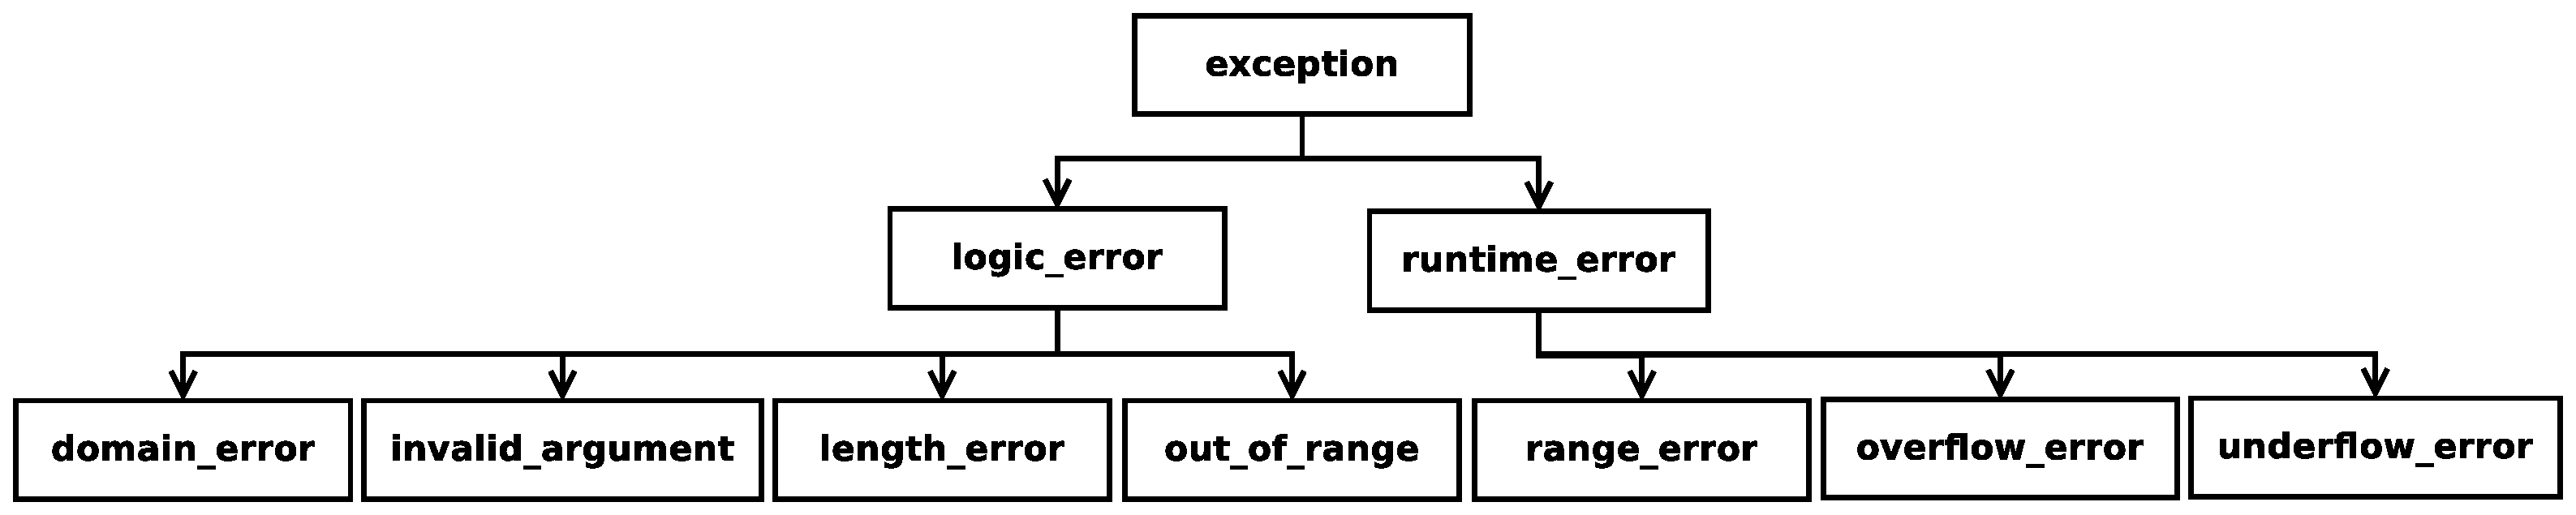
\includegraphics[scale=0.23]{figures/stdexcept.eps}
\caption{Diagram about the hierarchical structure of the \textit{stdexcept} library.}
\label{figure:stdexcept}
\end{figure*}

To define the types of errors in the \textit{stdexcept} library, we assume that
$e$ represents an element within the set $E$ such that for each $e$ exists one class
$\varphi$ that represents the error. Thus, $\varphi$ contains a constructor that sets an
error message to be thrown if there is an error during the program execution.
To identify these errors during the verification, whenever one of the
constructors of these classes is called, an $assert(0)$ is thrown, which forces ESBMC++ to
identify this error and report it in the counter-example. Note that ESBMC++
does not handle those exception as explained in section~\ref{exception-handling}, this
decision was made based on the fact that those exception are thrown when the C++ program
contains errors that can be potentially harmful to an application. The operational model
of the \textit{stdexcept} library can thus represented as:

\begin{equation}
\label{kind-of-exceptions}
\left\{ \begin{array}{ll}
              logic, domain, invalid\_argument, length, out\_of\_range,\\ runtime, range, overflow, underflow
        \end{array} \right\} \subset E
\end{equation}


\begin{equation}
\label{stdexcept}
\left( e \in E \right)
\Rightarrow \left(\forall e\right)\left(\exists\varphi\right)\left(\left(e\equiv\varphi\right)
\Rightarrow assert\left(0\right)\right)
\end{equation}

The category \textit{general libraries} also includes definitions
about the manipulation of characters sequences. Such definitions
are implemented in the \textit{string} library. In our operational
model, we implemented the main features of the \textit{string}
library through the iterator class that contains the
representation of the iterator for strings. In general,
we define the string object as an array of \textit{char} so that all
heuristics that must be observed in handling arrays are therefore
treated in this model. The main operations implemented by this library
are restricted to creation, insertion, deletion and search of elements
inside to object string.

As an example, we describe the implementation of the creation and search
operations. Firstly, we assume $S$ as the set of string variables,
$\eta$ as $NULL$ element, $c$ as a non-deterministic character,
the set $\left\{n, i, pos, length\right\} \subset N$,
and we define that $s$ represents a string, which has two attributes:
the string size described by $length$ and a character sequence that
represents it described by $str$. A constructor method can be defined
that creates a string containing $n$ times the character $c$. The method
\textit{find} that searches a character within a certain string from a
given position described by $pos$. We can thus model the $constructor$
of the string library as:
%
\begin{equation}
\label{constructor-string}
C := \left [ \begin{array}{ll}
                str_{1} = store\left(str_{0}, i_{0}, c_{0}\right) \\
		\wedge i_{1} = i_{0} + 1  \\
		\ldots \\
		\wedge \, \, str_{n} = store\left(str_{n-1}, i_{n-1}, c_{0}\right)
              \end{array} \right ],  \\
P := \left [ \begin{array}{ll}
                \left(i_{0} \geq 0\right)  \, \, \wedge \, \, \left(i_{0} < \left(n_{0} + 1\right)\right)\\
                \ldots \\
                \wedge \, \, \left(i_{n} \geq 0\right)  \, \, \wedge \, \, \left(i_{n} < \left(n_{0} + 1\right)\right)\\
                \wedge \, \, c_{0} \neq \eta\\
                \wedge \, \, n_{0} > 0\\
              \end{array} \right ]  \\
\end{equation}

The $find$ method can be modeled as:

\begin{equation}
\label{cfind-string}
C := \left [ \begin{array}{ll}
              found_{0} = ite\left(select\left(str, pos_{0}\right) = c_{0}, pos_{0}, -1\right)\\
              \ldots \\
               \wedge \, \, found_{n-1} = ite\left(select\left(str, pos_{n-1}\right) = c_{0}, pos_{n-1}, -1\right)\\
              \end{array} \right ],  \\
\nonumber
\end{equation}

\begin{equation}
\label{cfind-string-p}
P := \left [ \begin{array}{ll}
				 \left(c_{0} \neq \eta\right) \\
	       \left(pos_{0} \leq 0\right) \\
         \wedge \, \, \left(pos_{0} < length\right)\\
	       \ldots \\
	       \wedge \, \, \left(pos_{n-1} \leq 0\right)\\
	       \wedge \, \, \left(pos_{n-1} < length\right)\\

              \end{array} \right ]  \\
\end{equation}
}
%------------------------------------------------
\section{Inheritance and Polymorphism}
\label{inheritance-and-polymorphism}
%------------------------------------------------

Modeling C++ features like inheritance and polymorphism
makes static analysis difficult to implement.
\comment{
Inheritance is one of the main benefits of object-oriented paradigm,
which allows a class (derived class) absorbs data and behavior
from existing classes (base class) and thus enhances it with new features.
This is the vital concept behind the creation of reusable software components
and has received much attention because it is one of the promising ways to
improve software quality.}
In contrast to Java, which only allows single inheritance, where derived classes have only one base
class, C++ also allows multiple inheritance, where a class may inherit from one
or more unrelated base classes. This particular feature makes C++ programs
harder to model check than programs in other object-oriented programming
languages (e.g., Java). In this case, we have to replicate the methods and attributes of the base
classes to the inherited class to have direct access to them,
which thus disallows the direct use of tools already created
to other programming languages.

If a class inherits from a base class that does not contain virtual methods,
then we call this as \textit{replicated inheritance}. If there is a path from
class X to class Y whose first edge is virtual, then we call this as \textit{shared inheritance}.
A formal description to represent the relationship between the classes
can be described by the class hierarchy graph (CHG). This graph $\zeta$ is composed of a tuple
$ \textless \textbf{C}, \prec_{s}, \prec_{r}>$, \textbf{C} is the set of classes,
$\prec_s $ refers to shared inheritance edges, and $\prec_r$ are replicated inheritance edge.
$\prec_{s}$ and $\prec_{r}$ are the set of edges that represent inheritance relationship between
classes and $\subseteq \textbf{C} \times \textbf{C}$.
$\prec_{sr} = \prec_s \bigcup \prec_r$ and $\leq_{sr} = (\prec_{sr})^*$. ($\textbf{C}, \leq_{sr}$)
are a partially ordered set and $\leq_{sr}$ is anti-symmetric.

As an example, Figure~\ref{figure:uml_diagram} shows an UML diagram
that represents the \textit{Shape} class hierarchy, that contains multiple inheritance.
The Rectangle class relation can be formalized by
($\left(C, \left\langle Rectangle, Shape \right\rangle \right)$,
$\left(C, \left\langle Rectangle, Display \right\rangle \right)$).
Our tool creates an intermediate representation (IR) for single and multiple inheritance, handling
replicated and shared inheritance, see Figure~\ref{figure:multiple-inheritance-IR}.

\begin{figure}[ht]
\centering
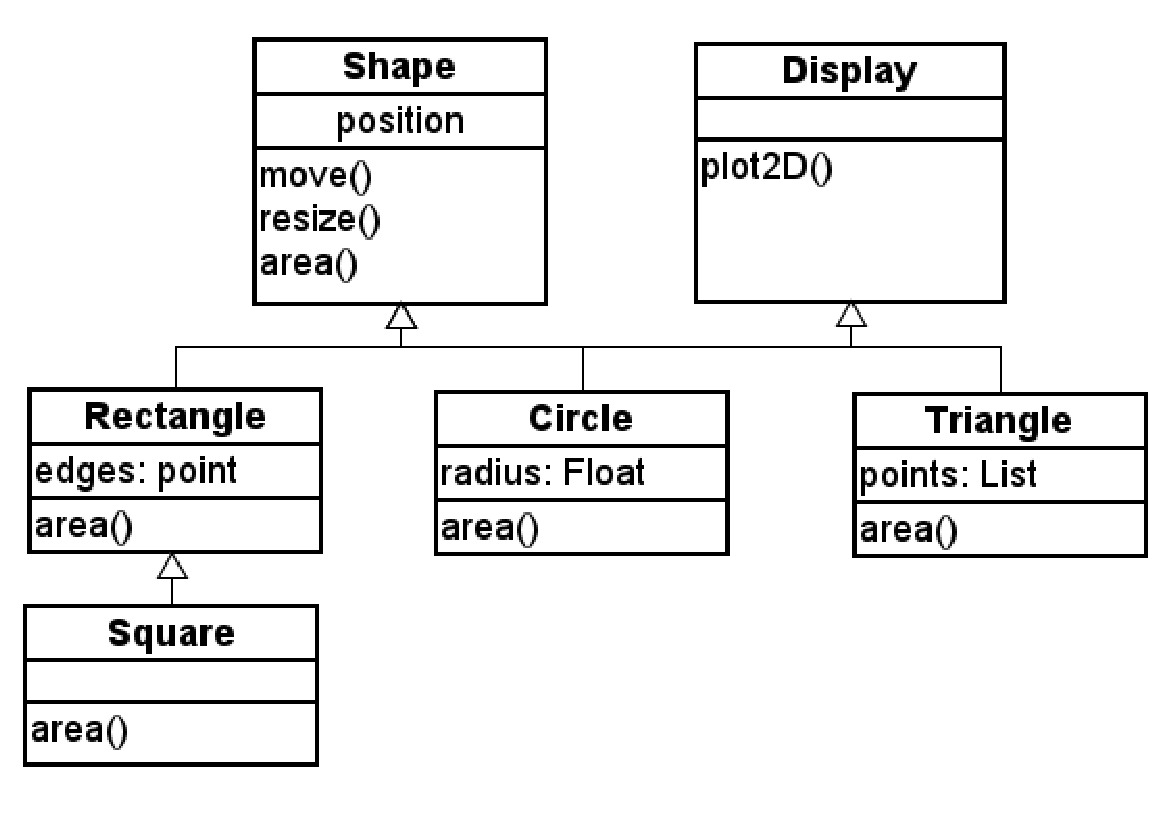
\includegraphics[scale=0.4]{figures/inheritance_uml}
\caption{Shape class hierarchy UML diagram}
\label{figure:uml_diagram}
\end{figure}


\begin{figure}[h]
\centering
\begin{minipage}{0.9\textwidth}
\begin{lstlisting}[style=nonumbers]
cpp::struct.Rectangle
    type:  struct
      * name: cpp::struct.Rectangle
components:
        0: name: cpp::struct.Shape::@vtable_pointer
        1: name: cpp::struct.Display::@vtable_pointer
        2: name: cpp::struct.Rectangle::@vtable_pointer
\end{lstlisting}
\end{minipage}
\caption{Multiple Inheritance: Intermediate Representation}
\label{figure:multiple-inheritance-IR}
\end{figure}

This model transforms all the classes in structures and joins all
methods and attributes of its parent classes. This approach has
the advantage of having direct access to the attributes and methods
of the derived class and thus allows an easier validation, as the tool
does not look for attributes or methods from base classes on each access.
On the other hand, we replicate information to any new class, thus wasting
memory resources.

Another important feature from object-oriented programing that our tool
supports is the concept of polymorphism. Polymorphism allows variable instances to be
bounded to references of different types according to the structure of the
inheritance hierarchy~\cite{Alexander02}.
It is the principle whereby two or more derived classes from the same base
class can invoke methods with same signature but distinct behaviors, specialized
for each derived class, using for this one reference to each object of this base class type.
The decision of which method must be used, according to the type of the
derived class, is chosen in run-time using the late binding.

The advantage is the creation of reusable code by programmers by changing only
specific features from the base class.

The intermediate representation provides a model to treat polymorphism in
order to simplify the class hierarchy,
easing the access to methods with the same name without ambiguity between
base and derived classes.
Our tool can handle the polymorphic area method using this representation,
as shown in Figure~\ref{figure:IR_uml_rec}.

Our tool also supports the indirect inheritance, which is a class that
inherits features from a derived class with one or more classes
not directly connected. In Figure~\ref{figure:uml_diagram}, \linebreak
$\left(C, \left\langle Square, Rectangle, Shape \right\rangle \right)$
thus Square class can access features from \textit{Shape} class,
but they are not directly connected. We tackle this problem by
looking for the features using depth search from the derived to base classes
and adding them to our intermediate representation if necessary,
as shown in Figure~\ref{figure:IR_uml_square}.


\begin{figure}[h]
\centering
\begin{minipage}{0.9\textwidth}
\begin{lstlisting}[style=nonumbers]
cpp::struct.Rectangle
    type:  struct
      * name: cpp::struct.Rectangle
methods:
        0: name: cpp::struct.Shape::area(this)
        1: name: cpp::struct.Display::plot2D(this)
        2: name: cpp::struct.Rectangle::area(this)
\end{lstlisting}
\end{minipage}
\caption{Intermediate Representation of Rectangle class}
\label{figure:IR_uml_rec}
\end{figure}


\begin{figure}[h]
\centering
\begin{minipage}{0.9\textwidth}
\begin{lstlisting}[style=nonumbers]
cpp::struct.Square
    type:  struct
      * name: cpp::struct.Square
methods:
        0: name: cpp::struct.Shape::area(this)
        1: name: cpp::struct.Rectangle::area(this)
        2: name: cpp::struct.Square::area(this)
\end{lstlisting}
\end{minipage}
\caption{Intermediate Representation of Square class}
\label{figure:IR_uml_square}
\end{figure}

In OO programming, the use of \textit{shared inheritance} is very common.
In contrast to other approaches (e.g.,~\cite{Blanc07}), ESBMC++ is able to
verify this kind of inheritance. If a class has pure virtual methods only,
then this class does not contain implementation for these methods and they will
thus be implemented in the derived classes. Otherwise, if a class has only virtual
methods, it must contain an implementation for them or the verification will fail
with a ``conversion error''. ESBMC++ also handles virtual destructors successfully
and supports the default constructor creation. However, ESBMC++ currently does not
support dynamic cast.

%--------------------------------------------
\section{Exception Handling}
\label{exception-handling}
%--------------------------------------------

One of the features that C++ provides is the exception handling. The exceptions are unexpected situations on the program, situations
that the program was not designed to handle. Basically, the exception handling is divided into three elements: a try block, where an
exception may occur, a catch block, where an exception can be handled and a throw expression to connect the two blocks. The
Figure~\ref{figure:try-catch-example} shows an example of a C++ code with exception handling.

\begin{figure}[ht]
\centering
\begin{minipage}{1.0\textwidth}
\begin{lstlisting}
int main() {
  try { // try block
    throw 20; // throw expression
  }
  // catch block
  catch (int i) { /* error handling for integer exceptions */ }
  catch (float f) { /* error handling for float exceptions */ }
  return 0;
}
\end{lstlisting}
\end{minipage}
\caption{Try-catch example: Throwing an integer exception.}
\label{figure:try-catch-example}
\end{figure}

On ESBMC++, the exception handling happens on two steps:
during the typechecking phase and the symbolic execution phase.
On the typechecking phase, an AST is built based on the code
inside the try block, with a few adaptations: before the code
inside the try block starts, a CATCH instruction with a empty map
(which will be filled later on the typechecking) is inserted, followed by
the code inside the try block, another CATCH instruction
(to represent the end of the try block and the beginning of the
catch block) and a GOTO instruction pointing to the code after
the catch block. This GOTO will only change if an exception is thrown,
otherwise it will remain the same. After typechecking the try block,
ESBMC++ typechecks the catch block that will contain one or more catchs.
Again, the AST will be created by based on the code inside the catchs
with only one adaptation: a GOTO instruction is inserted by the end of
each catch code pointing to the code after the catchs. Each catch code
will receive a label so ESBMC++ can decide which catch should be called
during the symbolic execution phase if an exception is thrown. By the end
of the catch block verification, the map of the first CATCH instruction
inserted before the try block code is filled with the label created
for each catch mapped on the type of exception. The Figure~\ref{figure:try-catch-goto}
shows the internal flow on ESBMC++ for exception handling of the code from
Figure~\ref{figure:try-catch-example}.

\begin{figure}[ht]
\centering
\begin{minipage}{1.0\textwidth}
\begin{lstlisting}
main() (c::main):
   CATCH signed_int->1, float->2
   THROW 20
   $TARGET = 3;
   if(THROW_TYPE == signed_int)
     $TARGET = 1
   else if(THROW_TYPE == float)
     $TARGET = 2
   CATCH
   GOTO $TARGET
1: int i;
   /* error handling for integer exceptions */
   GOTO 3
2: float f;
   /* error handling for float exceptions */
3: return 0;
END_FUNCTION
\end{lstlisting}
\end{minipage}
\caption{Try-catch conversion to goto functions.}
\label{figure:try-catch-goto}
\end{figure}

During the symbolic execution phase, when the first
CATCH instruction is found, the catch map is stacked
for later usage. The idea behind using a stack is
that we may have try-catch blocks inside other
try-catchs block and ESBMC++ should always handle
the most internal first. Following the symbolic execution
for the code that was inside the try block, ESBMC++ will continue
until it finds a throw expression. When this happens, ESBMC++ will
look at the map for a valid catch for the exception thrown, if it finds
a valid catch, the label will be saved for now and handled later;
if it was unable to find an exception an error will be shown.
ESBMC++ will also ignore any other throw or goto instruction after
the first throw is found but will continue to verify all the try
block code. When the second CATCH is found, which means that the try
block ended, the catch map is unstacked for memory efficiency
and the GOTO instruction is updated (if needed).

%------------------------------------------------------
\subsection{Throwing and Catching an Exception}
%------------------------------------------------------

A C++ code can throw an exceptions in several situations other
than explicit throw exception: (a) the new operator can throw a \textit{bad\_alloc}
exception, (b) the operator \textit{dynamic$\_$cast} can throw \textit{bad\_catch}
exception and the \textit{typeid} funtion can throw \textit{bad\_typeid} exception.
Those exceptions are built-in on C++ and are supposed to be handled by the program.
On the C++ draft standard~\cite{CppDraft} several rules are defined of how an exception
thrown is connected to a catch (called handlers), every time an exception is thrown and
one of the following rules is true, the code will jump from the throw expression to the catch code:

\begin{itemize}
 \item The handler that will catch the exception will be the first catch with a matching type: ESBMC++ maintains a list with the order of
       the catchs and always gets the catch with the lower value.
 \item A handler will catch an exception thrown if the type thrown and the type of the handler are the same (ignoring const-volatile
       qualifiers: ESBMC++ simply looks for the type of the exception in the catch map and update the GOTO instruction if it founds a
       match or returns an error otherwise).
 \item Throwing ''arrays of type T'' and ''functions returning type T'' with be catched by handlers with ''pointer to type T'' and
       ''pointer to function returning type T'' types: the conversion is made on the type-checking phase and the throw expression throws
       two exceptions: ''array of type T'' and ''pointer of type T'', and ''function returning type T'' and ''pointer to function returning
       type T'', respectively. The handler that will catch the exception thrown will be defined by the first rule in cases of multiple
       matches.
 \item The handler will catch an exception of type T if the handler type is an unambiguous public base class of T: The conversion is similar
       to the conversion of the last rule but in this case several exception may be thrown: the type of the object and the type of it's
       bases. Again, the handler will be defined by the first rule in cases of multiple matches.
 \item The handler will catch an exception of type pointer T if T's type can be converted to the type of the handler, either by
       qualification conversion or standard pointer conversion: Similar to the last rules, on the type-checking phase the possible
       conversions based on the catchs types will be thrown with the original pointer type, with the handler being defined by the first rule
       in cases of multiple matches.
 \item If the exception throw is a pointer then a handler with type \textit{void*} or \textit{nullptr\_t} can also catch it: during the symbolic execution phase, if no match is found on the map and the exception thrown is a pointer, we look for a \textit{void*} or \textit{nullptr\_t} catch and update the GOTO instruction. If the pointer had a match this rules is ignored.
 \item A handler of type ellipsis (...) will catch any thrown exception, and shall be the last handler on the catch block: Similar to the
       last rule but works for every type, if no match is found, ESBMC++ looks for a handler of type ellipsis and update the GOTO
       instruction if one exists.
\end{itemize}

%------------------------------------------------------
\subsection{Rethrows}
%------------------------------------------------------

Another feature that C++ provides for exception handling is the rethrow. The rethrow is an expression formed by
a throw with no argument. The rethrow function is to throw the last thrown exception so it can be handled further. To handle rethrows,
ESBMC++ always keeps a pointer to the last thrown exception and when it finds an throw without arguments (rethrow) it checks if this pointer
is not NULL, if it is NULL than the code is trying to rethrow an exception without a previous throw. If the pointer is not NULL than we have
a valid last thrown exception and the rethrow expression is replaced by a throw expression with the last expection as argument.

%------------------------------------------------------
\subsection{Exception Specification}
%------------------------------------------------------

The exception specifications define which exceptions a function or method (including constructors
and destructors) can throw. Alongside a method or function declaration a throw expression containing the exceptions list can define none or
multiple exceptions, which will forbid that any exception that is not in the exception specification to go out the function or method. Note
that an exception can still be handled inside a try-catch block inside the function or method even if it isn't on the exception specification.

The exception specification is handled inside ESBMC++ by inserting a THROW\_DECL instruction after the declaration of each function or method.
On the symbolic execution phase, the exception specification is stacked and removed on the END\_FUNCTION instruction by the end of every
function or method. The idea for stacking the exception specification is the same for catch maps, ESBMC++ may find function calls to other
function and they may also have their own exception specifications. Finally, when an exception is thrown, ESBMC++ checks if there is an
exception specification currently valid and if the exception thrown is allowed to be thrown outside the function. If it is allowed, the
exception handling follows and try to look for an match on the catch map or will return an error, otherwise.

%-----------------------------------
\section{Experimental Results}
%-----------------------------------

The experimental results is divided into two parts.
The setup is described in Section~\ref{experimental-setup}
while Section~\ref{comparison-to-LLBMC} describes a comparison
between ESBMC++\footnote{Available at http://esbmc.org/} and
LLBMC (Low-Level Bounded Model Checker)\footnote{Available at http://llbmc.org/}
using a set of standard C++ benchmarks. In our experiments, we also tried to
use the CBMC model checker~\cite{Clarke04}, but it has failed in most of our
benchmarks (as reported previously by Merz et~al.\~cite{Florian12}).

%-----------------------------------
\subsection{Experimental Setup}
\label{experimental-setup}
%-----------------------------------

The benchmark that are used in our comparison consist of 1113 C++ programs.
Around 290 programs are extracted from Deitel~\cite{Deitel},
16 programs are extracted from NEC~\cite{NeclabsBenchmarkExceptions},
16 programs are extracted from LLBMC~\cite{PrabhuMBIG11},
and the others were developed to test all the features that the C++ language
provides. The benchmarks are split into nine modules, as follows:
\textit{algorithm} contains test cases for methods that involve the
algorithm library; \textit{cpp} contains general test cases of the C++
language that involve the general libraries, multi-thread, and templates.
Additionally, it also contains the LLBMC's benchmarks and most of Deitel's
benchmarks are on this suite. The benchmarks \textit{deque}, \textit{list},
\textit{stream}, \textit{string}, and \textit{vector} contain test cases
related to deques, lists, stream, strings and vectors manipulations, respectively.
Finally, \textit{inheritance} contains test cases related to inheritance and
polymorphism while \textit{try\_catch} contains test cases related to exception handling
(NEC Labs' test cases are on this suite).

All the experiments were conducted on an otherwise idle Intel Core i7-2600,
3.40 GHz with 24 GB of RAM running Ubuntu 64-bits. For all the modules,
the individual time limit and memory limit for each test has been set to 900 seconds
and 24 GB (22 GB of RAM and 2 GB of virtual memory). The times given were measured
using the unix time command.

%-----------------------------------
\subsection{Comparison to LLBMC}
\label{comparison-to-LLBMC}
%-----------------------------------

This subsection describes the evaluation of ESBMC++ against another BMC tool developed by Merz et al.~\cite{Florian12}. Table~\ref{table:results-of-the-comparison-between-ESBMC-and-LLBMC} summarizes the results. Here, \textit{N} is the number of C++ programs, \textit{L} is the total lines of code of each suite, \textit{Time} is the total time of the verification of each module, \textit{P} is the number of positive results, \textit{FP} is the number of false positive results, \textit{FN} is the number of false negative results, \textit{Fail} is the number of internal errors during the verification of each module, \textit{TO} represents the number of time-outs ($>900$ seconds), and \textit{MO} represents the number of memory-outs ($>24$ GB).

\begin{table*}[t!]
\renewcommand\arraystretch{0.9}
\setlength{\tabcolsep}{4pt}
\begin{center} {\small
\begin{tabular}{|c|l|r|r||r|r|r|r|r|r|r|r|r|r|r|r|r|r|}
\hline
  & & & & \multicolumn{7}{c|}{ESBMC} & \multicolumn{7}{c|}{LLBMC} \\  \cline{5-18}
  & Testsuite & $N$ & $L$ & Time & P   & FP  & FN  & Crash & TO  & MO & Time & P   & FP  & FN  & Fail & TO  & MO \\\hline
1 & Algorithm & 127 & 3374 & 1697 & 96 & 21 & 10 & 0 & 0 & 0 & 23566 & 98 & 1 & 2 & 0 & 25 & 1\\ % OK
\hline
2 & Deque & 43 & 1239 & 1041 & 20 & 10 & 13 & 0 & 0 & 0 & 8580 & 33 & 0 & 0 & 1 & 9 & 0\\ % OK
\hline
3 & Vector & 146 & 6927 & 3263 & 137 & 3 & 6 & 0 & 0 & 0 & 7440 & 129 & 1 & 3 & 4 & 6 & 3\\ % OK
\hline
4 & List & 54 & 1731 & 316 & 18 & 23 & 13 & 0 & 0 & 0 & 1961 & 26 & 4 & 22 & 0 & 0 & 2\\ % OK
\hline
5 & Stream & 66 & 1828 & 2201 & 64 & 0 & 2 & 0 & 0 & 0 & 11 & 29 & 0 & 36 & 1 & 0 & 0\\ % OK
\hline
6 & String & 231 & 5022 & 19491 & 224& 5 & 2 & 0 & 0 & 0 & 28 & 122 & 4 & 105 & 0 & 0 & 0\\ % OK
\hline
7 & Inheritance & 40 & 3052 & 670 & 36 & 3 & 1 & 0 & 0 & 0 & 106 & 35 & 1 & 2 & 2 & 0 & 0\\ % OK
\hline
8 & Try\_catch & 67 & 4743 & 877 & 64 & 1 & 2 & 0 & 0 & 0 & 3 & 1 & 0 & 0 & 66 & 0 & 0 \\ % OK
\hline
9 & Cpp & 339 & 26720 & 3771 & 320 & 4 & 15 & 0 & 0 & 0 & 3992 & 261 & 7 & 52 & 15 & 3 & 1\\ % OK
\hline\hline
  &     &  1113 & 54636 & 33327 & 979 & 70 & 64 & 0 & 0 & 0 & 45687 & 734 & 18 & 222 & 89 & 43 & 7\\
\hline
\end{tabular} }
\end{center}
\caption{Results of the comparison between ESBMC v1.20 and LLBMC v2012.2.}
\label{table:results-of-the-comparison-between-ESBMC-and-LLBMC}
\end{table*}

The tool developed by Merz et al.~\cite{Florian12} is called LLBMC.
We invoked both tools using two scripts: one for ESBMC++, that reads
the parameters from a file and calls the tool
\footnote[1]{esbmc --unwind \textit{B} --no-unwinding-assertions -I ~/libraries/}
and another for LLBMC, that first compiles the code to bytecode using CLANG
\footnote[2]{/usr/bin/clang++ -c -g -emit-llvm *.cpp -fno-exceptions \newline /usr/bin/llvm-link *.o -o main.bc}~\cite{CLANG},
reads the parameters from a file and calls the tool\footnote[3]
{llbmc --ignore-missing-function-bodies --no-max-loop-iterations-checks --max-loop-iterations=\textit{B}}.
The bound set for both tools (value of \textit{B}) depends of each test case.
LLBMC currently does not support exception handling and all the bytecodes were generated without
exception support (flag -fno-exceptions) while verifying with LLBMC.
Enabling exceptions resulted in LLBMC aborting in most of the cases.

As we can see in Table ~\ref{table:results-of-the-comparison-between-ESBMC-and-LLBMC},
LLBMC time-outs 25 times in the algorithm module and runs out of memory in 1 test case.
Looking at those test cases, most of them use iterators, which maybe causing the slow down
on verification, a situation that repeats on others modules. On the Deque, Vector and List modules,
the slowdowns still happens but with small values. The module that had the most unsuccessful verification
results was the list module, and most of the errors were related to the container size
(e.g., assertions if the container is empty or if it has a particular size).
On ESBMC++, most of the errors on those modules are due to a missing operational model
of the libraries, which are currently under development.

On the stream module, most of the errors where related to assertions on the size
of the stream (using the method $gcount\left(\right)$) and to internal flags (such as
\textit{ios::hex} and \textit{iostream::hex}). On ESBMC++, most of the error were related
to bad operational model of internal flags. On the string module, the errors are related
to assertions on the string itself, usually if the string is equal to another string.
On Inheritance module, LLBMC reports some incorrect errors about memory write and
integer overflows while ESBMC++ failed on the verification of test cases involving
\textit{dynamic\_cast} (as described in Section~\ref{inheritance-and-polymorphism}).

On the \textit{try\_catch} module, LLBMC failed in most of the tests due to the fact that
the tool is missing support to exception handling. ESBMC++ was able to verify must of the cases.
The errors that occur are related to a missing implementation of exception specifications when
using classes constructors. And lastly, on the cpp module, which has test cases involving all
the others modules (but are not redundant), most of the errors presented were already seen during
the verification of others modules.

By the end, ESBMC++ verified the modules in 33327 seconds (approximately 9.25 hours) and successfully
verified 979 out of 1113 (~87.96\%) while LLBMC verified the modules in 45687 seconds (approximately 12.69 hours)
and successfully verified 734 out of 1113 (65.94\%). We can see that LLBMC is slower than ESBMC++ on the containers
and algorithm modules, while it is faster on stream and string modules but looses on successfully verified test cases.
On the inheritance module, the results of both tools are even.

On the \textit{try\_catch} module, ESBMC++ is able to verify almost all the tests,
something that LLBMC cannot due to its lack of support of exception handling. On the cpp module,
ESBMC++ is able to successfully verify many more test cases than LLBMC.
Also note that ESBMC++ does not crash, memory out or timeout in any module.

%-----------------------------------
\section{Related Work}
%-----------------------------------

Prabhu et al. presents an interprocedural exception
analysis and transformation framework for C++ that
records the control-flow created by the exceptions
and creates an exception-free program. The exception-free
program creation starts by generating a modular interprocedural
exception control-flow graph (IECFG). The IECFG is refined using
an algorithm based on a compact representation for a set of types
called the Signed-TypeSet domain and the result is used
to generate the exception-free program. Finally, the exception-free
program is verified using F-SOFT~\cite{Fsoft}. The verification is
focused on two properties: ``no throw'', the percentage of the code
that does not raise an exception and ``no leak'', the number memory
leaks on try-catch blocks.~\cite{PrabhuMBIG11}

Jing Yang et~al.\ present a translation tool called Class Hierarchy
Representation Object Model Extension (CHROME) that is targeted towards
making static program analyzers for C++ easier to write and provide
more precise results. CHROME makes a source-to-source transformation
from a C++ program with inheritance into a semantically equivalent without
inheritance by treating the inheritance as separate memory regions
that are linked to each other via additional base class and derived class
pointer fields. This transformation comprises a clarifier, which makes
implicit C++ features explicit. This approach was implemented with a bug
finding tool called F-SOFT~\cite{Fsoft}. CHROME has a
different memory behavior from the original program and therefore does not allow
the use of low-level primitives (e.g, \textit{memset}). The CHROME-lowered C program is
three to five times bigger than the size of the original C++ program ~\cite{Yang12}.

Blanc et~al.\ describes the verification of C++ programs (that use the STL containers)
via predicate abstraction~\cite{Blanc07}. They make use of abstract data types for the STL
usage verification rather than the actual STL implementation and behavior~\cite{Blanc07}.
Blanc et~al.\ show that it suffices to verify correctness using an operational model
by proving that the pre-conditions on operations in the model imply the pre-conditions
guaranteed by the language definition for those operations; similarly, the post-conditions
given by the standard imply the strongest post-conditions for the operational model.
This approach is very efficient in finding elemental errors in a C++ program, but it lacks
on a deeper seach for bugs and misleading operations (in particular, those that involve internal
modeling of the methods).

Merz et~al.\ describe the LLBMC tool, which also applies BMC to the verification
of C++ programs~\cite{Florian12}. However, they use the LLVM compiler to convert C++
programs into the LLVM's intermediate representation, which thus looses high-level
information about the structure of the C++ programs (i.e., the relationship between
the classes). Similarly to ESBMC++, Merz et~al.\ also apply SMT solvers to check the verification
conditions that are generated from the C++ programs. In contrast to our approach, however,
they do not handle exceptions, which thus make it difficult to verify realistic C++ programs
(e.g., programs that depend on the STL library).

Pasareanu and Visser developed a symbolic execution framework
for proving specifications of Java programs that contains loops,
also making use of invariant generation, strengthening and approximation
for discovering these loop invariants automatically~\cite{Pasareanu04}.
The invariant refinement gets close to the predicate abstraction concept,
by creating pre-conditions and Boolean expressions to verify the code validity.
It provides a stable technique that handles uniformly the different constraints.
Additionally, Pasareanu and Visser present a consistent verification and a high
flexible framework, but it is shares the lacks that predicate abstraction might
expose.

%------------------------------------------------------
\section{Conclusions}
%------------------------------------------------------

In this work, we have investigated SMT-based verification of C++ programs
by focusing on the major features that the language offers. We have described
an implementation of an operational model of the sequential STL containers
as well as novel approaches to handle inheritance, polymorphism and exception handling
(in particular, exception specification, which is a feature that is not supported by others
BMC tools). Our experiments consist of several test cases, which contain C++ programs
with most of the features that C++ language has to offer. The results show that
ESBMC++ outperforms LLBMC~\cite{Florian12} if we consider the verification of C++ programs.
ESBMC++ is also able to verify most of the test cases with an advantage: we are able to verify programs
with exceptions enabled (a missing feature of LLBMC that decreases the verification accuracy of
C++ programs). For future work, we intend to extend the operational model of STL containers
to support not only sequential containers but also mapped ones (e.g., map and multimap).

%\smallskip{\small\noindent{\bf Acknowledgments.}
%
%Acknowledgments here (Lucas)...
%}

\vspace{-2.5ex}
\renewcommand\refname{{\normalsize References}}
{\begin{thebibliography}{10}
\vspace{-0.5ex}

\bibitem{Bradley07}
A.~R. Bradley and Z.~Manna, \emph{The Calculus of Computation: Decision
  Procedures with Applications to Verification}.\hskip 1em plus 0.5em minus
  0.4em\relax Springer, 2007.

\bibitem{Wintersteiger09}
C.~Wintersteiger, \emph{Compiling GOTO-Programs},
  http://www.cprover.org/goto-cc/, 2009.

\bibitem{Sites74}
R.~L. Sites, ``Some thoughts on proving clean termination of programs.''
  Stanford, CA, USA, Tech. Rep., 1974.

\bibitem{PrabhuMBIG11}
P.~Prabhu, N.~Maeda, G.~Balakrishnan, F.~Ivancic, and A.~Gupta,
\newblock Interprocedural Exception Analysis for C++.
\newblock In {\em ECOOP}, pp. 583--608. 2011.

\bibitem{Pasareanu04}
C.~Pasareanu and W.~Visser,
\newblock Verification of Java Programs Using Symbolic Execution and Invariant
Generation.
\newblock In {\em SPIN}, LNCS 2989, pp. 164--181, 2004.

\bibitem{Blanc07}
N.~Blanc, A.~Groce, and D.~Kroening,
\newblock Verifying C++ with STL containers via predicate abstraction.
\newblock In {\em ASE}, pp. 521--524. 2007.

\bibitem{handbook09}
A.~Biere.
\newblock Bounded model checking.
\newblock In {\em Handbook of Satisfiability}, pp. 457--481. 2009.

\bibitem{Cimatti10}
A.~Cimatti, A.~Micheli, I.~Narasamdya, and M.~Roveri.
\newblock Verifying {SystemC}: a software model checking approach.
\newblock In {\em FMCAD}, 2010, pp.\ 121--128.

\bibitem{Clarke04}
E.~Clarke, D.~Kroening, and F.~Lerda.
\newblock A tool for checking {ANSI-C} programs.
\newblock In {\em TACAS}, {\em LNCS} 2988, pp.\ 168--176, 2004.

\bibitem{CordeiroPhD}
L.~Cordeiro.
\newblock {SMT}-Based Bounded Model Checking of Multi-Threaded Software in
Embedded Systems.
\newblock PhD Thesis, U Southampton, 2011.

\bibitem{icse11}
L.~Cordeiro and B.~Fischer.
\newblock Verifying Multi-Threaded Software using {SMT}-based Context-Bounded
Model Checking.
\newblock In {\em ICSE}, pp.\ 331--340, 2011.

\bibitem{sefm11}
J.~Morse, L.~Cordeiro, D.~Nicole, and B.~Fischer.
\newblock Context-Bounded Model Checking of LTL Properties for ANSI-C Software.
\newblock In {\em SEFM}, {\em LNCS} 7041, pp.\ 302--317, 2011.

\bibitem{Armando09}
A.~Armando, J.~Mantovani, and L.~Platania.
\newblock Bounded model checking of software using {SMT} solvers instead of
  {SAT} solvers.
\newblock In {\em STTT}, vol. 11 (1), pp. 69--83, 2009.

\bibitem{Ganai06}
M.~K. Ganai and A.~Gupta.
\newblock Accelerating high-level bounded model checking.
\newblock In {\em ICCAD}, pp. 794--801, 2006.

\bibitem{Cordeiro12}
L.~Cordeiro, B.~Fischer, and J.~Marques-Silva.
\newblock {SMT}-based bounded model checking for embedded {ANSI-C} software.
\newblock In {\em IEEE Trans. Software Eng.}, v.\ 38, n.\ 4, pp.\ 957--974, 2012.

\bibitem{Florian12}
F.~Merz, S.~Falke, and C.~Sinz.
\newblock {LLBMC}: Bounded Model Checking of C and C++ Programs Using a Compiler IR.
\newblock In {\em VSTTE}, pp.\ 146--161, 2012.

\bibitem{OpenCpp12}
OpenC++, http://opencxx.sourceforge.net/, 2012.

\bibitem{CppDraft}
C.standards commitee. Working draft, standard for programming language C++ (2012),
\newblock {http://www.open-std.org/JTC1/SC22/WG21/docs/papers/2012/n3376.pdf (acessed 8 october, 2012)}

\bibitem{CppReference12}
Reference of the C++ Language Library, http://www.cplusplus.com/reference/, 2012.

\bibitem{Fsoft}
F.~Ivancic, I.~Shlyakhter, A.~Gupta, M.~Ganai, V.~Kahlon, C.~Wang, Z.~Yang.
\newblock {Model Checking C programs using F-Soft.}
\newblock In {\em ICCD.} pp.\ 297--308, 2005.

\bibitem{CVC07}
C.~Barrett and C.~Tinelli, {CVC}3.
\newblock {\em CAV}, LNCS 4590, pp. 298--302, 2007.

\bibitem{smtlib09}
{SMT}-LIB, \emph{The Satisfiability Modulo Theories Library},
  http://combination.cs.uiowa.edu/smtlib, 2009.

\bibitem{McCarthy62}
J.~Mccarthy, ``Towards a mathematical science of computation,'' in \emph{
  IFIP Congress}.\hskip 1em plus 0.5em minus 0.4em\relax North-Holland,
  pp. 21--28, 1962.

\bibitem{Boolector09}
R.~Brummayer and A.~Biere, Boolector: An efficient {SMT} solver for  bit-vectors and arrays.
\newblock In {\em TACAS}, LNCS 5505, pp. 174--177, 2009.

\bibitem{Z08}
L.~M. de~Moura and N.~Bj{\o}rner, Z3: An efficient {SMT} solver.
\newblock In {\em  TACAS}, LNCS 4963, pp. 337--340, 2008.

\bibitem{Yang12}
J.~Yang, G.~Balakrishman, N.~Maeda, F.~Ivan\v{c}i\'c, A.~Gupta, N.~Sinha, S.~Sankaranarayanan and N.~Sharma.
\newblock {Object Model Construction for Inheritance in C++ and its Applications to Program Analysis.}
\newblock In {\em CC}, LNCS 7210, pp. 144--164, 2012.

\bibitem{Deitel}
P.~Deitel, H.~Deitel
\newblock {C++ How to Program}
\newblock Prentice Hall, 5th Edition, 2006.

\bibitem{Alexander02}
R. T.~Alexander, J.~Offutt and J. M.~Bieman. .
\newblock {Fault Detection Capabilities of Coupling-based OO Testing}
\newblock In {\em ISSRE '02} pp.~207--2002, 2002.

\bibitem{NeclabsBenchmarkExceptions}
NEC, http://www.nec-labs.com/research/system/systems\_SAV-website/benchmarks.php, 2012.

\bibitem{CLANG}
LLVM Tools, http://llvm.org/releases/, 2012.

\end{thebibliography}}

\end{document}

